\chapter{my first shader}
\label{sec:listing}
\lstset{style=68KStyle}

The busy heart of the \icode{texter} shader is its \icode{textloop}. This is a simple, but not especially short, piece of code that
will write an individual character to the screen, dilating, distorting and deforming it as required. The \icode{textloop} will
keep doing this until the string in \icode{textptr} runs out of characters, i.e. hits a \icode{\$00} byte such as at the end of
\icode{ataricop1}:

\begin{lstlisting}
ataricop1: dc.b "COPYRIGHT 1981,",0
\end{lstlisting}

This 'have we run out of characters to paint' logic is at the very start of the loop:

\begin{lstlisting}
textloop:
  loadb (textptr),r0 ; Put our text in r0.
  movei #ntxt,r1     ; Put our cleanup-and-exit routine in r1.
  addq #1,textptr    ; Move to the next character in textptr
  cmpq #0,r0         ; Check if it's $00
  jump eq,(r1)       ; If it is, jump to our cleanup-and-exit routine.
\end{lstlisting}

In this instance \icode{textptr} is pointing to \icode{ataricop1}. As soon as we hit the \icode{0} at the very end we will
\icode{jump} to \icode{ntxt}, which still stop the shader and bail out - unless 'drop shadow' mode was selected: in which
case it will paint the string a second time (slightly offset) to achieve the dropshadow effect:

\begin{lstlisting}[caption=In fact there is no offset for drop-shadow mode implemented\, so the feature is unused.  I suspect this is because the code is copy-pasted from elsewhere\,
as we shall encounter a cousin of this routine later on.]
ntxt:
  cmpq #1,mode       ; In drop-shadow mode?
  jr ne,StopGPU      ; No, bail.
  nop
  moveq #0,mode      ; Turn off drop-shadow flag so we bail next time.
  movei #textloop,r0 ; Put our textloop routine in r0.
  movefa r6,textptr  ; Rest textptr to the start of the string.
  movefa r7,dstxy    ; Reset our destination position to its original.
  jump (r0)          ; Jump to r0 (textloop)
\end{lstlisting}

Actually stopping the GPU involves clearing its command set to zero and loading that to the command register:
\begin{lstlisting}
StopGPU:
  movei #G_CTRL,r1   ; Get our GPU commands.
  load (r1),r0       ; Load them to r0.
  bclr #0,r0         ; Clear the GPU flags in r0 to make it stop.
  store r0,(r1)      ; Actually stop the GPU by loading the cleared flags.
stoploop:
  jr stoploop        ; Spin until the GPU actually stops.
\end{lstlisting}

Now that we see how our loop through the text starts and exits, we will obviously be curious to know how the 'writing
to the screen' part is effected. This is nearly identical to the method we stepped through for the 'Blitter'. The moment
that pixels are written to the screen is in these statements at the end of \icode{textloop}:

\begin{lstlisting}
  movei #(SRCEN|CLIP_A1|UPDA1F|UPDA1|UPDA2|LFU_A|LFU_AN|DCOMPEN),r0
  ...
  store r0,(blit)    ;draw the sprite
\end{lstlisting}

Here \icode{blit} is the equivalent of the \icode{B\_CMD} register we encountered in blitting. This is defined earlier on in the routine:
\begin{lstlisting}
  movei #B_CMD,blit   ; Use blit as an alias for B_CMD
\end{lstlisting}

By writing the contents of the
\icode{r0} register to \icode{blit} we are initiating a paint to the screen using all of the data we have setup earlier in the loop. This leads
naturally to the question: what data? Well, not unlike 'Blitting' we set up a bunch of parameters and data points defining our 'source' (\icode{A1}) and
our 'destination'(\icode{A2}). For both, these parameters and data points are concerned with things like positon, dimensions, screen width, and so on, not
to mention where we are going to get the pixels for drawing from (in our case we already know that this is going to be from \icode{pic}, the variable
point to the contents of \icode{beasty4.cry}).

We'll see how this data is calculated and derived shortly but first we'll take a look at the parameters and data points that are fed to the GPU and how.
Below we have the GPU blitter registers that control the way our pixel data is written to the screen, in the order in which our \icode{texter} routine
writes them:
\begin{figure}[H]
  {
    \setlength{\tabcolsep}{3.0pt}
    \setlength\cmidrulewidth{\heavyrulewidth} % Make cmidrule = 
    \begin{adjustbox}{width=12cm,center}

      \begin{tabular}{lllll}
        \toprule
        Common Name & T2K Name & Address in GPU RAM & Sample Value & Description\\
        \midrule
        \icode{A1\_PIXEL}   & \icode{a1\_n+\_pixel}  &\icode{\$F0220C} & \icode{00000001} & Current X Position in the Pixel Data\\
        \icode{A1\_FPIXEL}  & \icode{a1\_n+\_nfpixel} &\icode{\$F02218} & \icode{00000001} & Current Y Position in the Pixel Data\\
        \icode{A1\_STEP}  & \icode{a1\_n+\_step} &\icode{\$F02210} & \icode{00000001} & Current Y Position in the Pixel Data\\
        \icode{A1\_FSTEP}  & \icode{a1\_n+\_fstep} &\icode{\$F02214} & \icode{00000001} & Current Y Position in the Pixel Data\\
        \icode{A1\_INC}  & \icode{a1\_n+\_inc} &\icode{\$F0221C} & \icode{00000001} & Current Y Position in the Pixel Data\\
        \icode{A1\_FINC}  & \icode{a1\_n+\_finc} &\icode{\$F02220} & \icode{00000001} & Current Y Position in the Pixel Data\\
        \icode{A1\_FLAGS}  & \icode{a1\_n+\_flags} &\icode{\$F02204} & \icode{00000001} & Current Y Position in the Pixel Data\\
        \icode{A1\_BASE}  & \icode{a1\_n} &\icode{\$F02200} & \icode{00000001} & Current Y Position in the Pixel Data\\
        \icode{A1\_CLIP}  & \icode{a1\_n+\_clip} &\icode{\$F02208} & \icode{00000001} & Current Y Position in the Pixel Data\\
        \bottomrule
      \end{tabular}
    \end{adjustbox}
  }\caption*{The GPU blitter registers in the order in which \icode{texter} populates them in the listing below.}
\end{figure}

And here is the relevant code in the \icode{texter} populating the registers:

\begin{lstlisting}
  blit     REGEQU r13
  a1_n     REGEQU r14
  a2_n     REGEQU r15
  ...
rex:
  ...
  movei #A1_BASE,a1_n                        ; Make a1_n A1_BASE
  ...
  store xx,(a1_n+_pixel)                     ; Write to A1_PIXEL
  store yy,(a1_n+_fpixel)                    ; Write to A1_FPIXEL
  store r0,(a1_n+_step)                      ; Write to A1_STEP
  store r1,(a1_n+_fstep)                     ; Write to A1_FSTEP
  store xinc,(a1_n+_inc)                     ; Write to A1_INC
  store yinc,(a1_n+_finc)                    ; Write to A1_FINC

  movei #gpu_screen,r0         ; Prep gpu_screen as our destination
  movei #(PITCH1|PIXEL16|WID384|XADDINC),r1  ; Prep r1 for A1_FLAGS
  load (r0),r31                              ; Store gpu_screen in r31

  store r1,(a1_n+_flags)                     ; Write flags to A1_FLAGS
  movei #$1180180,r1                         ; Prep clip value.
  store r31,(a1_n)                           ; Write gpu_screen to A1_BASE
  store r1,(a1_n+_clip)                      ; Write clip value to A1_CLIP
\end{lstlisting}

This takes care of how we want the pixels to be written. On the other side of the equation we have to define for the GPU how want the source data
in \icode{beasty7.cry} to be read. Here is the order in which \icode{texter} populates this other side of the scale:

\begin{figure}[H]
  {
    \setlength{\tabcolsep}{3.0pt}
    \setlength\cmidrulewidth{\heavyrulewidth} % Make cmidrule = 
    \begin{adjustbox}{width=13cm,center}

      \begin{tabular}{lllll}
        \toprule
        Common Name & T2K Name & Address in GPU RAM & Value & Description\\
        \midrule
        \icode{A2\_BASE}  & \icode{a2\_n} &\icode{\$F02224} & \icode{\_bass} & Address of the source data\\
        \icode{A2\_PIXEL}   & \icode{a2\_n+\_pixel}  &\icode{\$F02230} & \icode{spixel} & Address of the pixel data in \icode{pic5/beasty7.cry}\\
        \icode{A2\_STEP}  & \icode{a2\_n+\_step} &\icode{\$F02234} & Derived from \icode{ssize} & The X and Y values for stepping\\
        \icode{A2\_FLAGS}  & \icode{a2\_n+\_flags} &\icode{\$F02228} & Calculated & Current Y Position in the Pixel Data\\
        \bottomrule
      \end{tabular}
    \end{adjustbox}
  }\caption*{The GPU blitter registers in the order in which \icode{texter} populates them in the listing below.}
\end{figure}

And here we are doing the populating:

\begin{lstlisting}
  store _bass,(a2_n)                  ; Write source address to A2_BASE
  store spixel,(a2_n+_pixel)          ; Write pixel data address to A2_PIXEL
  move ssize,r0                       ; Calculate the step size
  and lomask,r0 
  neg r0
  and lomask,r0
  bset #16,r0                         ; Set the width of the character
  movei #(PITCH1|PIXEL16|WID320|XADDPIX),r1 ; Prep flags
  store r0,(a2_n+_step)               ; Write step size to A1_STEP 
  store r1,(a2_n+_flags)              ; Write flags to A1_FLAGS
\end{lstlisting}

So far we've worked backwards from writing to the screen and got to the point where we completed the necessary admin of stuffing our
source (\icode{A2}) and destination (\icode{A1}) registers with the necessary odds and ends the GPU needs to write a character of our string to the
screen.  We've even received some clue as to what some of this data may actually mean.

The value in \icode{\_bass} that we write to \icode{A2\_BASE} is the value at the very start of our \icode{afont} data structure, in other words \icode{pic2}, the contents
of \icode{beasty7.cry} where our font pixels live. This is the blob of data the GPU will index into for its pixels to actually paint:
\begin{lstlisting}
afont:  
  dc.l pic2      ; pixel data
\end{lstlisting}

We loaded this from the \icode{in\_buf} passed to \icode{texter} by first storing it in \icode{fontbase} and then passing it into \icode{\_bass}:
\begin{lstlisting}
  movei #in_buf,r0    ;load the parameters into registers
  load (r0),textptr    ;point at start of textstring
  addq #4,r0
  load (r0),fontbase    ;point to start of font datastructure
  ...
  load (fontbase),_bass
\end{lstlisting}

The value \icode{spixel} we write to \icode{A2\_PIXEL} is the X and Y position of the character we want to paint in \icode{beasty7.cry/pic2}. We get this
value by indexing the ASCII value of our current character into our \icode{afont} data structure. 

\begin{lstlisting}
textloop:
  loadb (textptr),r0 ; Put our text in r0.
  movei #ntxt,r1     ; Put our cleanup-and-exit routine in r1.
  addq #1,textptr    ; Move to the next character in textptr
  cmpq #0,r0         ; Check if it's $00
  jump eq,(r1)       ; If it is, jump to our cleanup-and-exit routine.
  nop                ; It's no zero so we can get the x/y value for it from afont.
  subq #32,r0        ;ASCII 0-31 do NOT print
  shlq #2,r0
  add fontbase,r0    ; Add the fontbase address to our offset so we get the
                     ; actual address afont
  load (r0),spixel   ; Write the actual address to spixel.
\end{lstlisting}

In the above, if our character is \icode{A}, for example, this will result in us pulling out the following entry in \icode{afont}
\begin{lstlisting}
afont:
  ...
	dc.l $a40001	;A
\end{lstlisting}

As we saw earlier this contains the Y (\icode{a4}) and X (\icode{01}) position of our \icode{A} character in the \icode{beasty7.cry} image:

\begin{figure}[H]
    \centering
    \begin{adjustbox}{width=7.5cm,center}
      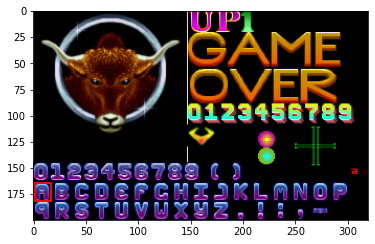
\includegraphics[width=12cm]{src/characters/plot.png}%
    \end{adjustbox}
\caption{The 'A' glyph located in a red box by our dimension and co-ordinate information.}
\end{figure}
